\title{Model}

{{navbar}}

\subsubsection{Model}

A probabilistic model is a joint distribution $p(\mathbf{x},
\mathbf{z})$ of data $\mathbf{x}$ and latent variables $\mathbf{z}$.
For background, see the \href{/tutorials/model}{Probabilistic Models tutorial}.

In Edward, we specify models using a simple language of random variables.
A random variable $\mathbf{x}$ is an object parameterized by
tensors $\theta^*$, where
the number of random variables in one object is determined by
the dimensions of its parameters.

\begin{lstlisting}[language=Python]
from edward.models import Normal, Exponential

# univariate normal
Normal(loc=tf.constant(0.0), scale=tf.constant(1.0))
# vector of 5 univariate normals
Normal(loc=tf.zeros(5), scale=tf.ones(5))
# 2 x 3 matrix of Exponentials
Exponential(rate=tf.ones([2, 3]))
\end{lstlisting}

For multivariate distributions, the multivariate dimension is the
innermost (right-most) dimension of the parameters.

\begin{lstlisting}[language=Python]
from edward.models import Dirichlet, MultivariateNormalTriL

# K-dimensional Dirichlet
Dirichlet(concentration=tf.constant([0.1] * K))
# vector of 5 K-dimensional multivariate normals with lower triangular cov
MultivariateNormalTriL(loc=tf.zeros([5, K]), scale_tril=tf.ones([5, K, K]))
# 2 x 5 matrix of K-dimensional multivariate normals
MultivariateNormalTriL(loc=tf.zeros([2, 5, K]), scale_tril=tf.ones([2, 5, K, K]))
\end{lstlisting}

Random variables are equipped with methods such as
\texttt{log_prob()}, $\log p(\mathbf{x}\mid\theta^*)$,
\texttt{mean()}, $\mathbb{E}_{p(\mathbf{x}\mid\theta^*)}[\mathbf{x}]$,
and \texttt{sample()}, $\mathbf{x}^*\sim p(\mathbf{x}\mid\theta^*)$.
Further, each random variable is associated to a tensor $\mathbf{x}^*$ in the
computational graph, which represents a single sample $\mathbf{x}^*\sim
p(\mathbf{x}\mid\theta^*)$.

This makes it easy to parameterize random variables with complex
deterministic structure, such as with deep neural networks, a diverse
set of math operations, and compatibility with third party libraries
which also build on TensorFlow.
The design also enables compositions of random variables
to capture complex stochastic structure.
They operate on $\mathbf{x}^*$.

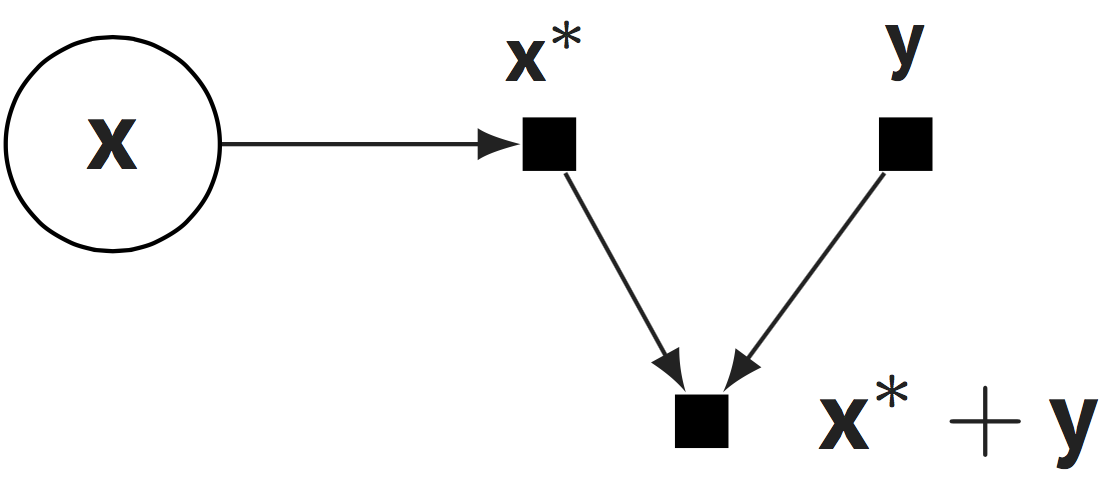
\includegraphics[width=375px]{/images/random_variable_ops.png}

\begin{lstlisting}[language=Python]
from edward.models import Normal

x = Normal(loc=tf.zeros(10), scale=tf.ones(10))
y = tf.constant(5.0)
x + y, x - y, x * y, x / y
tf.tanh(x * y)
x[2]  # 3rd normal rv in the vector
\end{lstlisting}

In the \href{/api/model-compositionality}{compositionality page}, we
describe how to build models by composing random variables.

\begin{center}\rule{3in}{0.4pt}\end{center}

For a list of random variables supported in Edward, see the
\href{/api/reference}{API reference page}.
Edward random variables build on top of them, inheriting the same
arguments and class methods. Additional methods are also available,
detailed below.


